
%%
%% This is file `sample-sigconf.tex',
%% generated with the docstrip utility.
%%
%% The original source files were:
%%
%% samples.dtx  (with options: `sigconf')
%% 
%% IMPORTANT NOTICE:
%% 
%% For the copyright see the source file.
%% 
%% Any modified versions of this file must be renamed
%% with new filenames distinct from sample-sigconf.tex.
%% 
%% For distribution of the original source see the terms
%% for copying and modification in the file samples.dtx.
%% 
%% This generated file may be distributed as long as the
%% original source files, as listed above, are part of the
%% same distribution. (The sources need not necessarily be
%% in the same archive or directory.)
%%
%% The first command in your LaTeX source must be the \documentclass command.
\documentclass[sigconf]{acmart}
\graphicspath{ {./imgs/} }
%%
%% \BibTeX command to typeset BibTeX logo in the docs
\AtBeginDocument{%
  \providecommand\BibTeX{{%
    \normalfont B\kern-0.5em{\scshape i\kern-0.25em b}\kern-0.8em\TeX}}}

%% Rights management information.  This information is sent to you
%% when you complete the rights form.  These commands have SAMPLE
%% values in them; it is your responsibility as an author to replace
%% the commands and values with those provided to you when you
%% complete the rights form.
%%\setcopyright{acmcopyright}
%%\copyrightyear{2018}
%%\acmYear{2018}
%%\acmDOI{10.1145/1122445.1122456}

%% These commands are for a PROCEEDINGS abstract or paper.
%%\acmConference[Woodstock '18]{Woodstock '18: ACM Symposium on Neural
%%  Gaze Detection}{June 03--05, 2018}{Woodstock, NY}
%%\acmBooktitle{Woodstock '18: ACM Symposium on Neural Gaze Detection,
%%  June 03--05, 2018, Woodstock, NY}
%%\acmPrice{15.00}
%%\acmISBN{978-1-4503-XXXX-X/18/06}


%%
%% Submission ID.
%% Use this when submitting an article to a sponsored event. You'll
%% receive a unique submission ID from the organizers
%% of the event, and this ID should be used as the parameter to this command.
%%\acmSubmissionID{123-A56-BU3}

%%
%% The majority of ACM publications use numbered citations and
%% references.  The command \citestyle{authoryear} switches to the
%% "author year" style.
%%
%% If you are preparing content for an event
%% sponsored by ACM SIGGRAPH, you must use the "author year" style of
%% citations and references.
%% Uncommenting
%% the next command will enable that style.
%%\citestyle{acmauthoryear}

%%
%% end of the preamble, start of the body of the document source.
\begin{document}

%%
%% The "title" command has an optional parameter,
%% allowing the author to define a "short title" to be used in page headers.
\title{Vulnerabilities in WebAssembly: A Survey}

%%
%% The "author" command and its associated commands are used to define
%% the authors and their affiliations.
%% Of note is the shared affiliation of the first two authors, and the
%% "authornote" and "authornotemark" commands
%% used to denote shared contribution to the research.
\author{Holger Klein}
%%\authornote{Both authors contributed equally to this research.}
%%\email{uaidx@student.kit.edu}
%%\orcid{1234-5678-9012}
%%\author{G.K.M. Tobin}
%%\authornotemark[1]
%%\email{webmaster@marysville-ohio.com}
\affiliation{%
  \institution{Karlsruhe Institute of Technology (KIT)}
%%  \streetaddress{P.O. Box 1212}
  \city{Karlsruhe}
%%  \state{Deutschland}
  \country{Germany}
%%  \postcode{43017-6221}
}


%%
%% By default, the full list of authors will be used in the page
%% headers. Often, this list is too long, and will overlap
%% other information printed in the page headers. This command allows
%% the author to define a more concise list
%% of authors' names for this purpose.
\renewcommand{\shortauthors}{Holger Klein}

%%
%% The abstract is a short summary of the work to be presented in the
%% article.
\begin{abstract}
  A clear and well-documented \LaTeX\ document is presented as an
  article formatted for publication by ACM in a conference proceedings
  or journal publication. Based on the ``acmart'' document class, this
  article presents and explains many of the common variations, as well
  as many of the formatting elements an author may use in the
  preparation of the documentation of their work.
\end{abstract}

%%
%% The code below is generated by the tool at http://dl.acm.org/ccs.cfm.
%% Please copy and paste the code instead of the example below.
%%

%%
%% Keywords. The author(s) should pick words that accurately describe
%% the work being presented. Separate the keywords with commas.
\keywords{binary exploits, Webassembly, IT Security}

%% A "teaser" image appears between the author and affiliation
%% information and the body of the document, and typically spans the
%% page.
\begin{teaserfigure}
  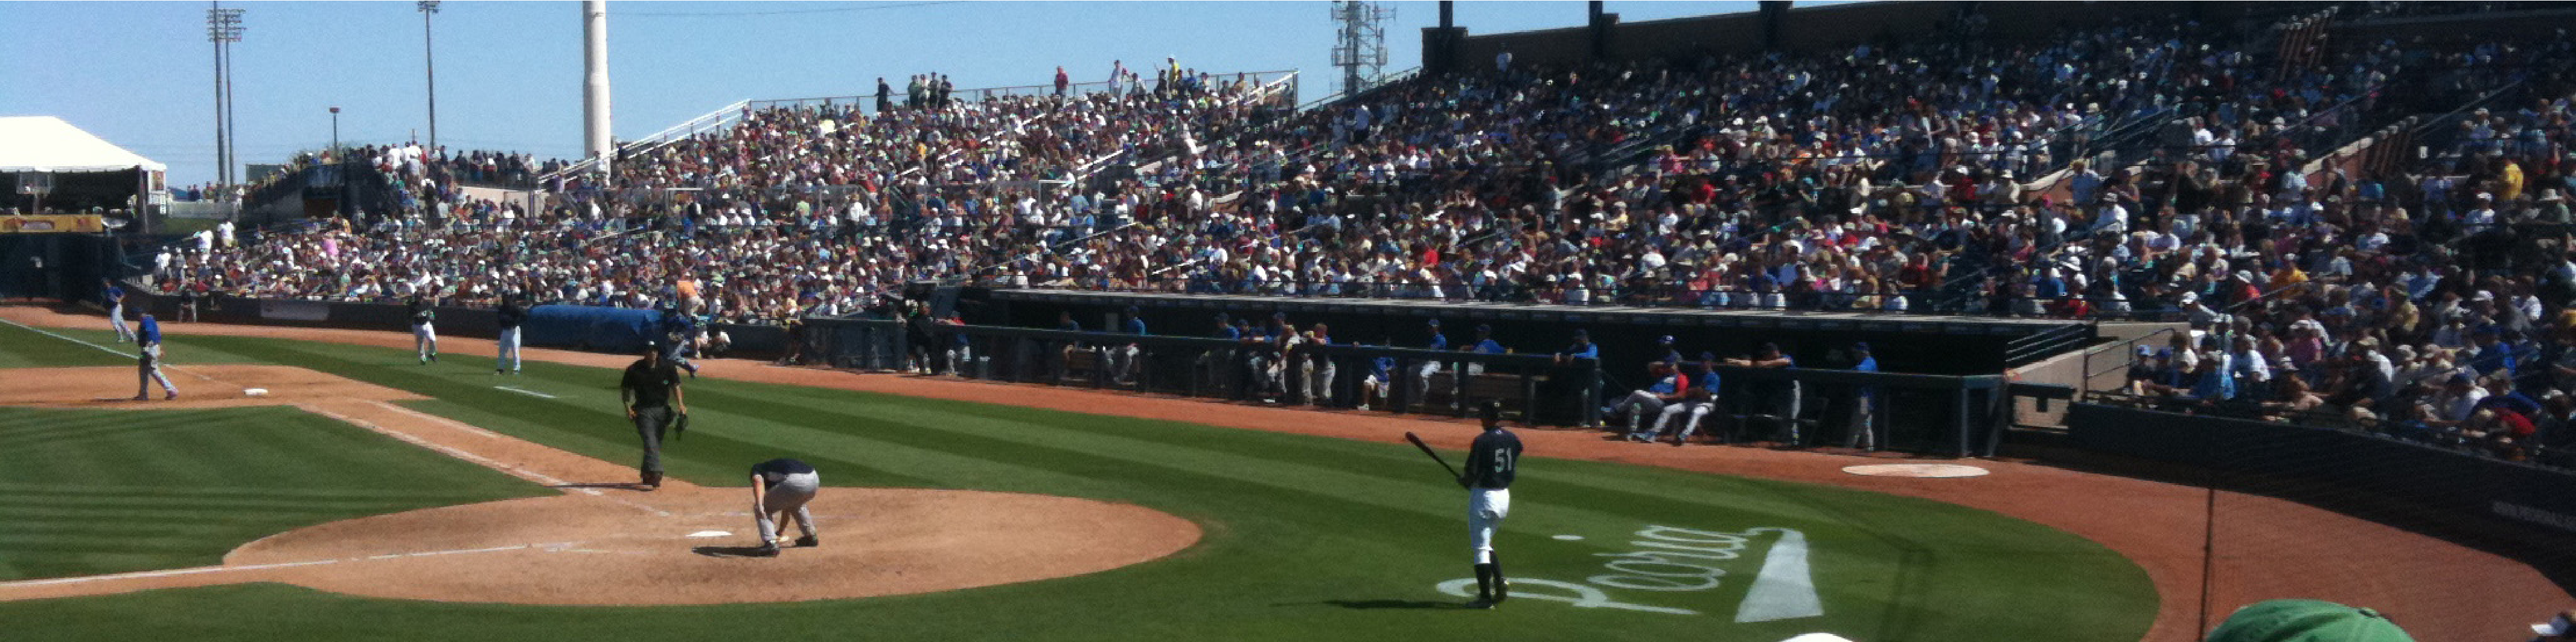
\includegraphics[width=\textwidth]{sampleteaser}
  \caption{Seattle Mariners at Spring Training, 2010.}
  \Description{Enjoying the baseball game from the third-base
  seats. Ichiro Suzuki preparing to bat.}
  \label{fig:teaser}
\end{teaserfigure}

%%
%% This command processes the author and affiliation and title
%% information and builds the first part of the formatted document.
\maketitle

\section{Introduction}
WebAssembly is a binary code format and compilation target meant to bring performance to web applications.  The initial design of the API and binary format of WebAssembly got completed in 2017 \cite{wasm_roadmap}. Since then, most major browsers such as Firefox, Chrome or Safari implement many of the proposed features. Even in the backend it is possible to run code compiled to WebAssembly for example when using Nodejs. The promise of running code with near native performance in the browser is very attractive, as it allows for more demanding web applications and smoother user experiences. However, since any Website visited by the user can download and execute WebAssembly code just like Javascript, it immediately raises security concerns. On the one hand, a malicious website could execute malware on the host PC or use computing ressources by executing a crypto miner. On the other hand, a vulnerable WebAssembly program which takes user input could lead to cross site scripting attacks in the browser. Worse yet, as WebAssebly gets adopted in the backend or even in stand-alone applications, vulnerabilities in WebAssembly programs could enable attacks such as Remote Code Execution. This survey will mainly deal with issues of the latter kind, focusing on how WebAssembly programs might be vulnerable to binary exploits. In particular, we will focus on how the security mechanisms intrinsic to WebAssembly's design compare to binary exploit mitigations in native applications. 
The official spec adresses some of the security concerns by stating that "[...] code is validated and executes in a memory-safe*, sandboxed environment preventing data corruption or security breaches". However, it adds a footnote which specifies "*No program can break WebAssembly’s memory model. Of course, it cannot guarantee that an unsafe language compiling to WebAssembly does not corrupt its own memory layout, e.g. inside WebAssembly’s linear memory". Indeed, in the past years there have been a few puplications commenting on WebAssembly's lack of mitigations to common binary exploitation techniques, such as \cite{mcfadden_security_2018} or \cite{lehmann_everything_2020}. Additionally, there have been puplications researching the use and existence of security vulnerabilities in real-world assembly programs such as \cite{hilbig_empirical_2021} or \cite{musch_new_2019}.  

\section{WebAssembly}
The following will give an Introduction to and and overview of Webassembly, paying special attention to the parts relevant to a discussion of binary vulnerabilities. For more information, see the official specification at \cite{webAssembly_spec_2021}. 

\subsubsection{High Level Overview}
The name 'WebAssembly' (often abbreviated as WASM) is a slight misnomer, since it has a different form and function from typical assembly languages. The official spec refers to it as "low-level, assembly-like". It is a binary byte code format which is interpreted by a Virtual Machine, similar to for example Java. The Virtual Machine is most often implemented in a browser. Design goals were to make WebAssembly safe, hardware- and language independent and fast. In fact, WebAssembly is supposed to run at near-native speeds. There exists a human-readable format of WebAssembly binaries called 'wat'. Whenever we present WebAssembly Code, it will be in this format. While it is possible to hand-craft wasm binary, it is most often generated by compiling a high-level language such as C/C++ or Rust. The Binary is then instantiated by calling a Javascript function. See \ref{fig:wasm_init_firefox}. WebAssembly functionality is then accessed by calling functions which are exported by the WebAssembly module from Javascript. WebAssembly has no I/O other than what is directly supplied through imported Javascript functions.

\begin{figure}[h]
  \centering
  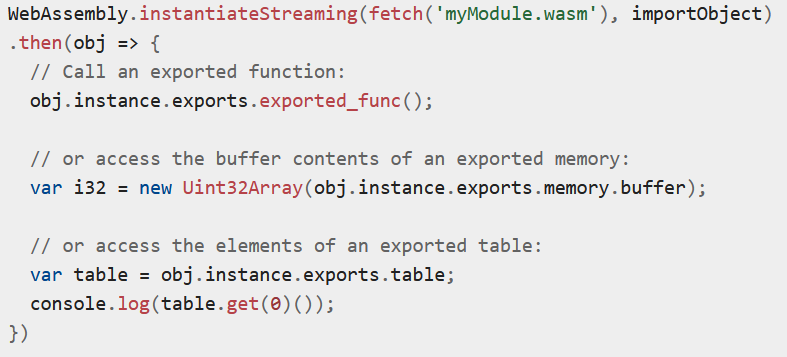
\includegraphics[width=\textwidth]{wasm_init_firefox}
  \caption{How to intantiate a WebAssembly module using Javascript. (\url{https://developer.mozilla.org/en-US/docs/WebAssembly/Loading_and_running}).}
\end{figure}


\subsubsection{Modules}
At the highest level, WebAssembly programs are organized into Modules.  


\bibliographystyle{ACM-Reference-Format}
\bibliography{Wasm-Vuln}

%%
%% If your work has an appendix, this is the place to put it.
\appendix


\end{document}
\endinput
%%
%% End of file `sample-sigconf.tex'.'